\documentclass[11pt]{article}
\usepackage{amsmath, amssymb, amsthm}
\usepackage{bm}
\usepackage{mathtools}
\usepackage{algorithm}
\usepackage{algpseudocode}
\usepackage{geometry}
\usepackage{hyperref}
\usepackage{xcolor}
\usepackage{booktabs}
\usepackage{tikz}
\usetikzlibrary{arrows.meta, positioning, shapes, shapes.geometric}
\definecolor{amber}{RGB}{180,120,10}

\geometry{margin=1in}

\theoremstyle{definition}
\newtheorem{definition}{Definition}[section]
\newtheorem{proposition}{Proposition}[section]
\newtheorem{remark}{Remark}[section]

\newcommand{\vz}{\mathbf{z}}
\newcommand{\vy}{\mathbf{y}}
\newcommand{\ve}{\mathbf{e}}
\newcommand{\vx}{\mathbf{x}}
\newcommand{\W}{\mathbf{W}}
\newcommand{\R}{\mathbf{R}}
\newcommand{\E}{\mathbf{E}}
\newcommand{\A}{\mathbf{A}}
\newcommand{\B}{\mathbf{B}}
\newcommand{\mU}{\mathbf{U}}
\newcommand{\mS}{\mathbf{\Sigma}}
\newcommand{\mV}{\mathbf{V}}
\newcommand{\vU}{\mathbf{U}}
\newcommand{\vV}{\mathbf{V}}
\newcommand{\vH}{\mathbf{h}}
\newcommand{\rank}{\mathrm{rank}}
\newcommand{\diag}{\mathrm{diag}}
\newcommand{\tr}{\mathrm{tr}}
\newcommand{\Rbb}{\mathbb{R}}
\newcommand{\norm}[1]{\left\|#1\right\|}
\newcommand{\pderiv}[2]{\frac{\partial #1}{\partial #2}}
\newcommand{\pd}{\partial}

\title{\textbf{LRA and rec-LRA on the Parallel Temporal Neural Coding Network}\\
  \large Mathematical Derivations, Low-Rank Factorization, and Fast Weights Integration}
\author{Hitesh (Research Notes) \\ \small University of South Florida}
\date{\today}

\begin{document}
\maketitle
\tableofcontents
\newpage

%===============================================================================
\section{Background: The P-TNCN Architecture}
%===============================================================================

\subsection{Notation}

Let $L$ denote the total number of layers. At time step $t$, layer $\ell$
($1 \le \ell \le L$) maintains a state vector $\vz^\ell_t \in \Rbb^{d_\ell}$,
where $d_\ell$ is the hidden dimension of layer $\ell$ (often $d_\ell = d$
for all $\ell$ in the isotropic case). We denote:

\begin{itemize}
  \item $\W^\ell \in \Rbb^{d_\ell \times d_{\ell-1}}$: feedforward weight matrix at layer $\ell$
  \item $\R^\ell \in \Rbb^{d_\ell \times d_\ell}$: recurrent (lateral) weight matrix at layer $\ell$
  \item $\W^\ell_o \in \Rbb^{d_{\ell-1} \times d_\ell}$: output/prediction weight matrix
  \item $\E^\ell \in \Rbb^{d_\ell \times d_{\ell-1}}$: error synapse matrix at layer $\ell$
  \item $\phi(\cdot)$: element-wise nonlinear activation function (e.g., tanh, ReLU)
  \item $K$: number of inference correction steps per time step
  \item $\beta$: modulation factor for error signal transmission
\end{itemize}

\subsection{Forward Pass (Prediction Phase)}

Given input $\vx_t \in \Rbb^{d_0}$ and previous states
$\{\vz^\ell_{t-1}\}^L_{\ell=1}$, the P-TNCN computes:

\begin{equation}
  \label{eq:state_update}
  \vz^\ell_t = \phi\!\left(\W^\ell \vz^{\ell-1}_t + \R^\ell \vz^\ell_{t-1}\right),
  \quad \vz^0_t = \vx_t
\end{equation}

Each layer $\ell$ then generates a \emph{prediction} of the layer below:
\begin{equation}
  \label{eq:prediction}
  \vz^{\ell-1}_{t,o} = \phi\!\left(\W^{\ell-1}_o \, \vz^\ell_t\right)
\end{equation}

The prediction error (error unit) at layer $\ell-1$ is:
\begin{equation}
  \label{eq:error_unit}
  \ve^{\ell-1}_t = \vz^{\ell-1}_t - \vz^{\ell-1}_{t,o}
\end{equation}

\subsection{Inference Correction Phase ($K$ steps)}

The P-TNCN iteratively corrects its internal states using the error units.
Let $\vy^{\ell,(k)}_{t,z}$ denote the corrected state of layer $\ell$ at
inference step $k \in \{1,\ldots,K\}$. Starting from $\vy^{\ell,(0)}_{t,z} = \vz^\ell_t$:

\begin{equation}
  \label{eq:correction}
  \vy^{\ell,(k)}_{t,z} = \vz^\ell_t + \beta \cdot \E^\ell \, \ve^{\ell-1,(k-1)}_t
\end{equation}

where the error units are recomputed after each correction step:
\begin{equation}
  \ve^{\ell-1,(k)}_t = \vz^{\ell-1}_t - \phi\!\left(\W^{\ell-1}_o \, \vy^{\ell,(k)}_{t,z}\right)
\end{equation}

After $K$ steps, the final corrected state is $\vy^\ell_{t,z} \coloneqq \vy^{\ell,(K)}_{t,z}$.

\subsection{Local Weight Update Rules (LRA)}

The P-TNCN's synaptic weights are updated using a Hebbian-like local rule,
derived from minimizing the \emph{total discrepancy} functional:
\begin{equation}
  \label{eq:total_discrepancy}
  \mathcal{D}(\Theta) = \sum_{\ell=1}^{L} \lambda_\ell \norm{\vz^\ell_t - \vy^\ell_{t,z}}^2_2
\end{equation}

Taking partial derivatives and applying the discrepancy reduction framework
(Ororbia et al., 2020), the weight update rules are:

\begin{align}
  \Delta \W^\ell &= \left(\vy^\ell_{t,z} - \vz^\ell_t\right) \left(\vz^{\ell-1}_t\right)^\top \label{eq:dW} \\
  \Delta \R^\ell &= \left(\vy^\ell_{t,z} - \vz^\ell_t\right) \left(\vz^\ell_{t-1}\right)^\top \label{eq:dR} \\
  \Delta \E^\ell &= -\alpha_E \cdot \vz^\ell_t \left(\ve^{\ell-1}_t\right)^\top \label{eq:dE}
\end{align}

where $\alpha_E < \alpha_W$ (error synapses updated more slowly than feedforward ones).

\begin{remark}
The updates in Equations~\eqref{eq:dW}--\eqref{eq:dE} are \textbf{purely local}:
each depends only on pre- and post-synaptic activities available at that layer.
No global error signal from the output layer is required. This is the key property
we must preserve when applying low-rank factorizations.
\end{remark}

%===============================================================================
\section{Local Representation Alignment (LRA) — Formal Specification}
%===============================================================================

\subsection{The Discrepancy Reduction Framework}

LRA operates by minimizing the total discrepancy $\mathcal{D}(\Theta)$ of
Equation~\eqref{eq:total_discrepancy}. The key insight is that each layer
$\ell$ has a \emph{target representation} $\vy^\ell_{t,z}$ that it should
have produced, and the weight updates align the layer's actual output with
this target using a Hebbian rule.

For a feedforward connection from layer $k$ to $\ell$ via weight $\W_{k \to \ell}$:
\begin{equation}
  \Delta \W_{k \to \ell} = \ve^\ell \cdot \left(\vz^k\right)^\top,
  \quad \text{where } \ve^\ell = \vy^\ell_{t,z} - \vz^\ell_t
\end{equation}

For the error synapses $\E_{j \to \ell}$ that route error signals from layer $j$ to $\ell$:
\begin{equation}
  \Delta \E_{j \to \ell} = -\gamma \left(\vz^\ell \cdot (\ve^j)^\top\right)
\end{equation}

where $\gamma \ll \alpha_W$ slows the error synapse evolution.

\subsection{Recursive LRA (rec-LRA)}

Rec-LRA (Ororbia \& Mali, AAAI 2023) generalizes LRA to deep networks by
recursively computing targets layer-by-layer using \emph{skip-error connections}.
For layer $i$ with error neurons $\ve^i$, the target for an upstream layer $m$ is:

\begin{equation}
  \label{eq:reclra_target}
  \bm{\delta}^m = \beta \cdot \E_{i \to m} \cdot \ve^i
\end{equation}

\begin{equation}
  \label{eq:reclra_correction}
  \vy^m = \phi\!\left(\tilde{\vz}^m - \bm{\delta}^m\right), \quad \ve^m = \vy^m - \vz^m
\end{equation}

The recursion proceeds until all layers have been assigned a target. Weight
updates then follow the same Hebbian form. The total complexity is $O(Ld^2)$
per step — identical to LRA and linear in the number of layers.

\subsection{rec-LRA Applied to a Standard RNN}
\label{sec:reclra-rnn}

Before specialising to the P-TNCN, it is instructive to see how rec-LRA replaces
backpropagation-through-time (BPTT) in the simplest setting: a single-hidden-layer
RNN trained on next-token prediction.

\paragraph{Model.}
Let $\mathbf{h}_t \in \mathbb{R}^{d}$ denote the hidden state, $\mathbf{x}_t \in \mathbb{R}^{k}$
the input, and $\hat{\mathbf{y}}_t \in \mathbb{R}^{c}$ the predicted output distribution.
The forward pass is:
\begin{align}
  \mathbf{h}_t     &= \phi\!\left(\mathbf{W}\,\mathbf{h}_{t-1} + \mathbf{U}\,\mathbf{x}_t\right)
                      \label{eq:rnn_forward} \\
  \hat{\mathbf{y}}_t &= \mathrm{softmax}\!\left(\mathbf{V}\,\mathbf{h}_t\right)
                      \label{eq:rnn_output}
\end{align}
where $\mathbf{W} \in \mathbb{R}^{d \times d}$ is the recurrent matrix,
$\mathbf{U} \in \mathbb{R}^{d \times k}$ the input matrix, and
$\mathbf{V} \in \mathbb{R}^{c \times d}$ the output matrix.

\paragraph{Output error (Phase 2).}
Given the ground-truth one-hot vector $\mathbf{y}_t$, the output error neuron is:
\begin{equation}
  \mathbf{e}^{\mathrm{out}}_t = \mathbf{y}_t - \hat{\mathbf{y}}_t
  \label{eq:rnn_eout}
\end{equation}
\textbf{Contrast with backprop:} BPTT propagates this signal \emph{backwards} through
$\mathbf{V}^\top$, then through $\mathbf{W}^\top$ for every unrolled time step.
rec-LRA instead routes it through a \emph{separate, learnable} skip-error synapse
$\mathbf{E}_{L \to h} \in \mathbb{R}^{d \times c}$ — which can be optionally
factorised as $\mathbf{A}\mathbf{B}$ (rank $r$) — directly to the hidden layer.

\paragraph{rec-LRA correction (Phase 3).}
The displacement signal (perturbation) transmitted to the hidden layer is:
\begin{equation}
  \bm{\delta}_h = \mathbf{E}_{L \to h}\,\mathbf{e}^{\mathrm{out}}_t
  \label{eq:rnn_delta}
\end{equation}
The corrected (target) hidden state is then computed in a single step (no unrolling):
\begin{equation}
  \tilde{\mathbf{y}}_t = \phi\!\left(\tilde{\mathbf{h}}_t - \beta\,\bm{\delta}_h\right),
  \qquad \mathbf{e}^h_t = \tilde{\mathbf{y}}_t - \mathbf{h}_t
  \label{eq:rnn_corrected}
\end{equation}
where $\tilde{\mathbf{h}}_t = \mathbf{W}\,\mathbf{h}_{t-1} + \mathbf{U}\,\mathbf{x}_t$
is the pre-activation of $\mathbf{h}_t$, and $\mathbf{e}^h_t$ is the hidden-layer
correction residual analogous to $\ve^\ell_\mathrm{corr}$ in the P-TNCN.

\paragraph{Local weight updates (Phase 4).}
All parameter updates are Hebbian: each weight matrix is updated using only
quantities available at its two endpoint layers — no global chain rule required.
\begin{align}
  \Delta\mathbf{W}              &= \mathbf{e}^h_t\,\bigl(\mathbf{h}_{t-1}\bigr)^\top
                                   \label{eq:rnn_dW} \\
  \Delta\mathbf{U}              &= \mathbf{e}^h_t\,\bigl(\mathbf{x}_t\bigr)^\top
                                   \label{eq:rnn_dU} \\
  \Delta\mathbf{V}              &= \mathbf{e}^{\mathrm{out}}_t\,\bigl(\mathbf{h}_t\bigr)^\top
                                   \label{eq:rnn_dV} \\
  \Delta\mathbf{E}_{L \to h}    &= -\gamma\,\mathbf{h}_t\,\bigl(\mathbf{e}^{\mathrm{out}}_t\bigr)^\top
                                   \label{eq:rnn_dE}
\end{align}

\begin{remark}[No temporal unrolling]
Equations~\eqref{eq:rnn_dW}--\eqref{eq:rnn_dE} are computed \emph{at time $t$},
using only states from $t$ and $t{-}1$. There is no sum over past time steps,
no stored activation history, and no vanishing/exploding gradient through time.
The recurrent matrix $\mathbf{W}$ is updated by a single outer product of the
hidden correction residual and the previous hidden state.
\end{remark}

\begin{remark}[Key difference from BPTT]
BPTT computes $\partial \mathcal{L}/\partial \mathbf{W}$ by propagating a single
error signal backwards along the \emph{same} pathway ($\mathbf{V}^\top$,
$\mathbf{W}^\top$, ...) used in the forward pass — the weight transport problem.
rec-LRA uses a \emph{structurally distinct} skip-error pathway $\mathbf{E}_{L \to h}$
that is \emph{separately learned}, freeing it from weight symmetry and enabling
true layer-wise parallelism.
\end{remark}

\begin{figure}[h]
\centering
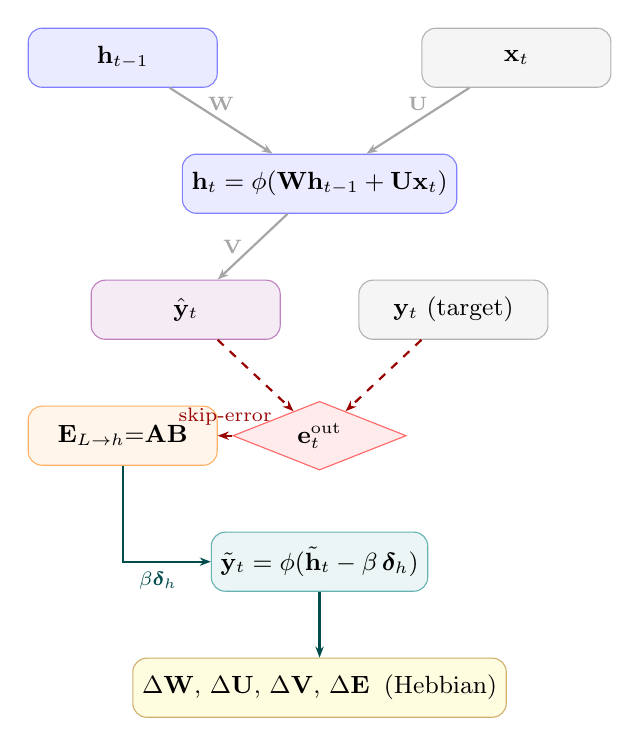
\begin{tikzpicture}[
  node distance = 0pt,
  box/.style     = {rectangle, draw=gray!60, fill=gray!8, rounded corners=5pt,
                    minimum width=2.4cm, minimum height=0.75cm, align=center,
                    font=\small},
  bluebox/.style = {box, draw=blue!50, fill=blue!8},
  purpbox/.style = {box, draw=violet!50, fill=violet!8},
  tealbox/.style = {box, draw=teal!60, fill=teal!8},
  coralbox/.style= {box, draw=orange!60, fill=orange!8},
  amberbox/.style= {box, draw=amber!60, fill=yellow!12},
  dia/.style     = {diamond, draw=red!60, fill=red!8, aspect=2.5,
                    minimum width=2.2cm, minimum height=0.8cm, align=center,
                    font=\small\bfseries},
  fwd/.style     = {-{Stealth[length=4pt]}, thick, gray!70},
  err/.style     = {-{Stealth[length=4pt]}, thick, red!60!black, dashed},
  cor/.style     = {-{Stealth[length=4pt]}, thick, teal!60!black}
]

\node[bluebox]  (hprev) at (0,   3.6) {$\mathbf{h}_{t-1}$};
\node[box]      (xt)    at (5.0, 3.6) {$\mathbf{x}_t$};
\node[bluebox]  (ht)    at (2.5, 2.0) {$\mathbf{h}_t = \phi(\mathbf{W}\mathbf{h}_{t-1}+\mathbf{U}\mathbf{x}_t)$};
\node[purpbox]  (yhat)  at (0.8, 0.4) {$\hat{\mathbf{y}}_t$};
\node[box]      (yt)    at (4.2, 0.4) {$\mathbf{y}_t$ (target)};
\node[dia]      (eout)  at (2.5,-1.2) {$\mathbf{e}^{\mathrm{out}}_t$};
\node[coralbox] (Emat)  at (0.0,-1.2) {$\mathbf{E}_{L\to h}{=}\mathbf{A}\mathbf{B}$};
\node[tealbox]  (ytil)  at (2.5,-2.8) {$\tilde{\mathbf{y}}_t = \phi(\tilde{\mathbf{h}}_t - \beta\,\bm{\delta}_h)$};
\node[amberbox] (upd)   at (2.5,-4.4) {$\Delta\mathbf{W},\,\Delta\mathbf{U},\,\Delta\mathbf{V},\,\Delta\mathbf{E}$\;\;(Hebbian)};

\draw[fwd] (hprev) -- node[above,font=\scriptsize]{$\mathbf{W}$} (ht);
\draw[fwd] (xt)    -- node[above,font=\scriptsize]{$\mathbf{U}$} (ht);
\draw[fwd] (ht)    -- node[left, font=\scriptsize]{$\mathbf{V}$} (yhat);
\draw[err] (yhat)  -- (eout);
\draw[err] (yt)    -- (eout);
\draw[err] (eout)  -- node[above,font=\scriptsize]{skip-error} (Emat);
\draw[cor] (Emat)  |- node[below,font=\scriptsize,pos=0.7]{$\beta\bm{\delta}_h$} (ytil);
\draw[cor] (ytil)  -- (upd);
\end{tikzpicture}
\caption{%
  rec-LRA applied to a single-hidden-layer RNN.
  \textbf{Blue}: hidden states updated by local Hebbian rules.
  \textbf{Red dashed}: error signals routed through the separate skip-error
  synapse $\mathbf{E}_{L \to h}$ (coral box, factorised as $\mathbf{A}\mathbf{B}$).
  \textbf{Teal}: corrected target state $\tilde{\mathbf{y}}_t$ used for all updates.
  No backpropagation through time is needed.
}
\label{fig:reclra-rnn}
\end{figure}

\paragraph{Comparison: rec-LRA vs.\ BPTT gradient for $\mathbf{W}$.}
Under BPTT, the gradient of the cross-entropy loss $\mathcal{L}$ with respect to
$\mathbf{W}$ at time step $t$ is:
\begin{equation}
  \nabla_{\mathbf{W}} \mathcal{L}
    = \sum_{\tau=1}^{t} \frac{\partial \mathcal{L}}{\partial \mathbf{h}_\tau}
      \left(\mathbf{h}_{\tau-1}\right)^\top,
  \quad \text{where }
  \frac{\partial \mathcal{L}}{\partial \mathbf{h}_\tau}
    = \mathbf{W}^\top \frac{\partial \mathcal{L}}{\partial \mathbf{h}_{\tau+1}}
      \odot \phi'(\mathbf{h}_\tau)
\end{equation}
This sum over $\tau$ is what causes BPTT to require storing the full activation
history and unrolling the graph. The rec-LRA update (Eq.~\eqref{eq:rnn_dW}):
\begin{equation}
  \Delta\mathbf{W} = \mathbf{e}^h_t\,\bigl(\mathbf{h}_{t-1}\bigr)^\top
\end{equation}
discards the temporal sum and uses only the \emph{current-step} correction
residual $\mathbf{e}^h_t = \tilde{\mathbf{y}}_t - \mathbf{h}_t$ as a proxy
for the true gradient. This is within $90^\circ$ of the true gradient direction
(Ororbia et al., 2020), ensuring the update still makes progress on the objective
while remaining online and history-free.

%===============================================================================
\section{Low-Rank Factorization of Error Synapses in P-TNCN}
%===============================================================================

\subsection{Motivation}

The error synapse matrix $\E^\ell \in \Rbb^{d \times d}$ introduces $d^2$
parameters per layer. For $d = 512$ and $L = 3$ layers, this adds $\approx 786$K
additional parameters beyond the forward weights. Empirically, error synapses
tend to be nearly low-rank after training (small effective rank), suggesting
that a factorized parameterization is both parameter-efficient and
mathematically justified.

\subsection{Factorized Error Synapses: $\E^\ell = \A^\ell \B^\ell$}

We propose replacing each full error synapse matrix with a low-rank factorization:
\begin{equation}
  \label{eq:lora_E}
  \E^\ell \approx \A^\ell \B^\ell, \quad \A^\ell \in \Rbb^{d \times r}, \quad \B^\ell \in \Rbb^{r \times d}
\end{equation}

where $r \ll d$ is the \emph{rank hyperparameter}. The parameter count for $\E^\ell$ reduces from $d^2$ to $2dr$.

\begin{definition}[LRA-PTNCN]
A P-TNCN where all error synapse matrices $\{\E^\ell\}_{\ell=1}^L$ are replaced
by rank-$r$ factorizations $\{\A^\ell \B^\ell\}_{\ell=1}^L$, with the local
Hebbian update rule adapted to update $\A^\ell$ and $\B^\ell$ independently.
\end{definition}

\subsection{Deriving Local Update Rules for $\A^\ell$ and $\B^\ell$}

Starting from the total discrepancy (Equation~\eqref{eq:total_discrepancy})
and substituting $\E^\ell = \A^\ell \B^\ell$:

\begin{equation}
  \mathcal{D} \supset \lambda_\ell \norm{\vz^\ell - \vy^\ell_{t,z}}^2_2
  = \lambda_\ell \norm{\vz^\ell - (\vz^\ell + \beta \A^\ell \B^\ell \ve^{\ell-1})}^2_2
\end{equation}

Computing partial derivatives:

\begin{align}
  \pderiv{\mathcal{D}}{\A^\ell}
    &= -2\lambda_\ell \beta \left(\vy^\ell_{t,z} - \vz^\ell\right) \left(\B^\ell \ve^{\ell-1}\right)^\top \\
    &= -2\lambda_\ell \beta \, \ve^\ell_\text{corr} \cdot \left(\B^\ell \ve^{\ell-1}\right)^\top
    \label{eq:dA}
\end{align}

\begin{align}
  \pderiv{\mathcal{D}}{\B^\ell}
    &= -2\lambda_\ell \beta \left(\A^\ell\right)^\top \left(\vy^\ell_{t,z} - \vz^\ell\right) \left(\ve^{\ell-1}\right)^\top \\
    &= -2\lambda_\ell \beta \left(\A^\ell\right)^\top \ve^\ell_\text{corr} \cdot \left(\ve^{\ell-1}\right)^\top
    \label{eq:dB}
\end{align}

where $\ve^\ell_\text{corr} \coloneqq \vy^\ell_{t,z} - \vz^\ell_t$ is the
\emph{correction residual} (how much the state had to be corrected).

\begin{proposition}[Locality of $\Delta\A^\ell$ and $\Delta\B^\ell$]
The updates in Equations~\eqref{eq:dA} and~\eqref{eq:dB} are local: $\Delta\A^\ell$
depends only on quantities available at layer $\ell$ ($\ve^\ell_\text{corr}$) and
a \emph{projected} version of the error from below ($\B^\ell \ve^{\ell-1}$), while
$\Delta\B^\ell$ depends on $(\A^\ell)^\top \ve^\ell_\text{corr}$ and $\ve^{\ell-1}$.
No backpropagation is required.
\end{proposition}

The Hebbian update rules therefore become:

\begin{equation}
  \boxed{
  \Delta \A^\ell = \alpha_A \, \ve^\ell_\text{corr} \cdot \left(\B^\ell \ve^{\ell-1}\right)^\top
  }
\end{equation}

\begin{equation}
  \boxed{
  \Delta \B^\ell = \alpha_B \, \left(\A^\ell\right)^\top \ve^\ell_\text{corr} \cdot \left(\ve^{\ell-1}\right)^\top
  }
\end{equation}

\subsection{Initialization Strategy}

\paragraph{Random initialization (baseline):}
$\A^\ell \sim \mathcal{N}(0, \sigma^2_A)$,
$\B^\ell = \mathbf{0}$, so that $\E^\ell = \A^\ell \B^\ell = \mathbf{0}$ initially.
This matches the common LoRA initialization (Hu et al., 2022).

\paragraph{SVD warm-start (recommended for fine-tuning):}
Given a pretrained full $\E^\ell$, compute its thin SVD:
$\E^\ell = \mU \mS \mV^\top$. Initialize:
\begin{equation}
  \A^\ell = \mU_{:, 1:r} \cdot \mS^{1/2}_{1:r,1:r}, \qquad
  \B^\ell = \mS^{1/2}_{1:r,1:r} \cdot \mV^\top_{:, 1:r}
\end{equation}

This preserves the top-$r$ modes of the original error routing structure.

\subsection{Effective Rank Analysis}

To monitor whether rank-$r$ is a sufficient approximation, we track the
\emph{stable rank} (or effective rank) of $\E^\ell$ during training:
\begin{equation}
  \text{srank}(\E^\ell) = \frac{\norm{\E^\ell}^2_F}{\norm{\E^\ell}^2_2}
  = \frac{\sum_i \sigma_i^2}{\sigma_{\max}^2}
\end{equation}

If $\text{srank}(\E^\ell) < r$ consistently, the rank $r$ is unnecessarily large.
If $\text{srank}(\E^\ell) \approx r$, we are at capacity and should increase $r$.

%===============================================================================
\section{Applying rec-LRA to P-TNCN: The rec-LRA-PTNCN Algorithm}
%===============================================================================

\subsection{Skip-Error Connections for Temporal Models}

In rec-LRA, error signals are not constrained to follow the feedforward
pathway backward. Instead, skip-error connections $\E_{j \to \ell}$ route
error information from any layer $j$ to any layer $\ell$. For the P-TNCN,
we extend this to the temporal domain:

\begin{equation}
  \label{eq:reclra_ptncn}
  \bm{\delta}^\ell_t = \sum_{j \in \mathcal{N}(\ell)} \E_{j \to \ell} \cdot \ve^j_t
\end{equation}

where $\mathcal{N}(\ell)$ is the set of source layers whose error neurons
connect to layer $\ell$'s correction circuit.

\begin{remark}[Temporal error routing]
In the P-TNCN, error signals are computed at time $t$ and used to correct
states at time $t$ (no temporal backtracking). Rec-LRA preserves this property:
skip-error connections only route across the depth axis, not across the time axis.
\end{remark}

\subsection{Full rec-LRA-PTNCN Update Algorithm}

\begin{algorithm}[H]
\caption{rec-LRA-PTNCN: One Time Step}
\label{alg:reclra_ptncn}
\begin{algorithmic}[1]
  \Require Input $\vx_t$, previous states $\{\vz^\ell_{t-1}\}_\ell$,
           parameters $\Theta = \{\W^\ell, \R^\ell, \W^\ell_o, \A^\ell, \B^\ell\}_\ell$
  \Ensure Updated states $\{\vy^\ell_{t,z}\}_\ell$, parameter updates $\Delta\Theta$

  \State \textbf{// Phase 1: Forward pass}
  \For{$\ell = 1$ to $L$}
    \State $\vz^\ell_t \gets \phi(\W^\ell \vz^{\ell-1}_t + \R^\ell \vz^\ell_{t-1})$
    \Comment{Eq.~\eqref{eq:state_update}}
    \State $\vz^{\ell-1}_{t,o} \gets \phi(\W^{\ell-1}_o \vz^\ell_t)$
    \Comment{Eq.~\eqref{eq:prediction}}
    \State $\ve^{\ell-1}_t \gets \vz^{\ell-1}_t - \vz^{\ell-1}_{t,o}$
    \Comment{Eq.~\eqref{eq:error_unit}}
  \EndFor

  \State \textbf{// Phase 2: Rec-LRA target generation (skip-error routing)}
  \State $\ve^L_t \gets \vz^L_t - \hat{\vx}_t$ \Comment{Output layer error}
  \For{$\ell = L-1$ downto $1$} \Comment{Recursive target propagation}
    \State $\bm{\delta}^\ell_t \gets \A^\ell \B^\ell \ve^\ell_t$
    \Comment{Low-rank error routing, Eq.~\eqref{eq:reclra_ptncn}}
    \State $\vy^\ell_{t,z} \gets \phi(\tilde{\vz}^\ell_t - \beta \bm{\delta}^\ell_t)$
    \State $\ve^\ell_\text{corr} \gets \vy^\ell_{t,z} - \vz^\ell_t$
  \EndFor

  \State \textbf{// Phase 3: Weight updates (all local, parallelizable)}
  \For{$\ell = 1$ to $L$} \Comment{Can run on separate GPUs}
    \State $\Delta\W^\ell \gets \ve^\ell_\text{corr} \cdot (\vz^{\ell-1}_t)^\top$
    \State $\Delta\R^\ell \gets \ve^\ell_\text{corr} \cdot (\vz^\ell_{t-1})^\top$
    \State $\Delta\A^\ell \gets \alpha_A \, \ve^\ell_\text{corr} \cdot (\B^\ell \ve^{\ell-1}_t)^\top$
    \State $\Delta\B^\ell \gets \alpha_B \, (\A^\ell)^\top \ve^\ell_\text{corr} \cdot (\ve^{\ell-1}_t)^\top$
  \EndFor
\end{algorithmic}
\end{algorithm}

\subsection{Parameter Count Comparison}

\begin{table}[h]
\centering
\begin{tabular}{lcc}
\toprule
\textbf{Model} & \textbf{E-matrix params} & \textbf{Total (d=512, L=3)} \\
\midrule
PTNCN (full E)       & $3 \times d^2 = 786$K    & $\approx 8.4$M \\
LRA-PTNCN (rank 8)   & $3 \times 2dr = 24.6$K   & $\approx 7.6$M \\
LRA-PTNCN (rank 32)  & $3 \times 2dr = 98.3$K   & $\approx 7.7$M \\
LRA-PTNCN (rank 128) & $3 \times 2dr = 393$K    & $\approx 8.0$M \\
\bottomrule
\end{tabular}
\caption{Parameter count for full vs. factorized error synapses ($d=512$, $L=3$).}
\end{table}

%===============================================================================
\section{Fast Weights Integration into P-TNCN}
%===============================================================================

\subsection{Fast Weight Mechanism (Ba et al., 2016)}

Fast weights maintain a rapidly-decaying Hebbian associative memory buffer
$\mathbf{F}_t \in \Rbb^{d \times d}$ that accumulates outer products of recent
hidden states:

\begin{equation}
  \label{eq:fast_weight_update}
  \mathbf{F}_t = \lambda \mathbf{F}_{t-1} + \eta \, \vz^\ell_t \left(\vz^\ell_t\right)^\top
\end{equation}

The fast weight buffer modulates the current state via:
\begin{equation}
  \label{eq:fast_weight_apply}
  \tilde{\vz}^\ell_t = \mathrm{LayerNorm}\!\left(\vz^\ell_t + \mathbf{F}_t \, \vz^\ell_t\right)
\end{equation}

where $\lambda \in [0, 1)$ is the decay factor and $\eta$ is the learning rate
for the fast weight buffer.

\subsection{Placement Options in P-TNCN}

We consider three distinct integration points for fast weights in the P-TNCN:

\paragraph{Option A (Post-state, pre-correction):}
Replace the state in the inference correction phase:
\begin{equation}
  \vy^{\ell,(k)}_{t,z} = \tilde{\vz}^\ell_t + \beta \E^\ell \ve^{\ell-1,(k-1)}_t
  \quad \text{where } \tilde{\vz}^\ell_t = \mathrm{LN}(\vz^\ell_t + \mathbf{F}^\ell_t \vz^\ell_t)
\end{equation}

\paragraph{Option B (Fast-weight modulated error unit):}
The error unit itself is modulated:
\begin{equation}
  \ve^{\ell-1}_t = \vz^{\ell-1}_t - \phi\!\left(\W^{\ell-1}_o \tilde{\vz}^\ell_t\right)
\end{equation}

\paragraph{Option C (Dynamic error synapse):}
The fast weight buffer serves as a dynamic, input-dependent component of $\E^\ell$:
\begin{equation}
  \E^\ell_t = \underbrace{\A^\ell \B^\ell}_{\text{slow, learned}} + \underbrace{\gamma \mathbf{F}^\ell_t}_{\text{fast, transient}}
\end{equation}

This is the most theoretically interesting option, as it allows the error routing
to adapt on-the-fly within a sequence without modifying slow-timescale weights.

\subsection{Hybrid Training: Backprop for Fast Weights, LRA for Slow Weights}

Since fast weights are differentiable with respect to their outputs, we can train them
using standard backpropagation while keeping the LRA updates for the slow weights:

\begin{equation}
  \text{Slow weights: } \{\W^\ell, \R^\ell, \A^\ell, \B^\ell\} \leftarrow \text{LRA update (local, no gradient)}
\end{equation}
\begin{equation}
  \text{Fast weight scalars: } \{\lambda, \eta, \gamma\} \leftarrow \nabla_{\theta_\text{fw}} \mathcal{L}_\text{NLL}(\theta_\text{fw})
\end{equation}

This hybrid is compatible with JAX: use `jax.lax.stop_gradient` on the LRA quantities
and allow JAX autodiff to flow through the fast weight computation.

\subsection{Interaction with Inference Correction}

A key question is whether the K-step inference correction and the fast weight
buffer are \emph{complementary} or \emph{redundant}:

\begin{itemize}
  \item The K-step correction operates \textbf{within} a single time step:
    it refines the current representation $\vz^\ell_t$ by iteratively reducing
    prediction error.
  \item The fast weight buffer operates \textbf{across} time steps:
    it stores a compressed, decaying memory of recent state trajectories.
\end{itemize}

We hypothesize that they are complementary: fast weights improve the initial
state estimate $\vz^\ell_t$, and the K-step correction then refines this
improved estimate. Formally, if $\tilde{\vz}^\ell_t$ (fast-weight-modulated)
has lower initial prediction error than $\vz^\ell_t$, then K fewer correction
steps should be needed to achieve the same BPC.

\begin{proposition}[Fast weight redundancy condition]
If the fast weight buffer $\mathbf{F}^\ell_t$ perfectly encodes the next-state
prediction (i.e., $\phi(\W^\ell_o \tilde{\vz}^\ell_t) = \vz^{\ell-1}_t$), then
$\ve^{\ell-1}_t = \mathbf{0}$ and the K-step correction has no effect. In this
limiting case, the fast weights fully subsume the inference correction.
\end{proposition}

This suggests an adaptive K schedule: reduce K when $\norm{\ve^{\ell-1}_t}_2$
is small (fast weights are working well) and increase K when it is large.

%===============================================================================
\section{JAX Implementation Notes}
%===============================================================================

\subsection{Why JAX?}

JAX is ideal for this project for several reasons:
\begin{itemize}
  \item \textbf{Functional purity}: JAX's explicit state management
    maps directly onto the P-TNCN's stateful but mathematically clean architecture.
  \item \textbf{JIT compilation}: \texttt{jax.jit} traces the computation graph
    and compiles it to XLA, giving CUDA-level performance from Python code.
  \item \textbf{vmap}: The K-step inference correction loop can be \texttt{vmap}'d
    over the batch dimension, enabling highly efficient parallel correction.
  \item \textbf{grad/value\_and\_grad}: For the hybrid training (fast weights via
    backprop), \texttt{jax.grad} provides automatic differentiation.
\end{itemize}

\subsection{Key JAX Patterns for This Project}

\paragraph{Stateful carry with \texttt{jax.lax.scan}:}
Time-step unrolling over a sequence uses \texttt{lax.scan} to avoid Python-level
loops (which JAX would unroll, bloating compilation time):

\begin{verbatim}
def step(carry, x_t):
    states, F = carry
    states, F, metrics = ptncn_step(states, F, x_t, params)
    return (states, F), metrics

(final_carry, all_metrics), _ = jax.lax.scan(step, init_carry, x_seq)
\end{verbatim}

\paragraph{Low-rank E update with \texttt{jax.jit}:}
The factorized update $\Delta\A = \ve_\text{corr} (\B \ve^{\ell-1})^\top$
is a rank-1 update scaled by residuals — this is efficient as a \texttt{jnp.outer}
or \texttt{jnp.einsum('i,j->ij', ...)}.

\paragraph{Stop-gradient for hybrid training:}
\begin{verbatim}
slow_weight_update = lra_update(jax.lax.stop_gradient(correction_residual))
fast_weight_loss = jnp.mean(nll_loss(model_with_fast_weights(x, params)))
fast_weight_grad = jax.grad(lambda fw: fast_weight_loss(fw))(fast_weights)
\end{verbatim}

%===============================================================================
\section{Experimental Protocol}
%===============================================================================

\subsection{Datasets}
\begin{itemize}
  \item \textbf{Penn Treebank (PTB)}: Standard character-level split.
    Train/val/test: 5.0M / 393K / 442K characters.
  \item \textbf{Text8}: Larger benchmark (100M characters) for scaling tests.
\end{itemize}

\subsection{Metrics}
\begin{itemize}
  \item \textbf{Bits-per-character (BPC)} = $\log_2 e \cdot \mathrm{NLL}$. Target: $< 1.43$ (PTB).
  \item \textbf{Effective rank} of $\E^\ell = \A^\ell \B^\ell$ (stable rank).
  \item \textbf{Correction residual norm}: $\frac{1}{L}\sum_\ell \norm{\ve^\ell_\text{corr}}_2$ (convergence of K steps).
\end{itemize}

\subsection{Ablation Matrix}

\begin{table}[h]
\centering
\begin{tabular}{lccccc}
\toprule
\textbf{Variant} & \textbf{E-rank} & \textbf{W-rank} & \textbf{Fast W.} & \textbf{Hybrid BP} & \textbf{Expected BPC} \\
\midrule
PTNCN-full (baseline)     & $d$   & $d$   & No  & No  & 1.43 \\
LRA-PTNCN-r8              & 8     & $d$   & No  & No  & TBD  \\
LRA-PTNCN-r32             & 32    & $d$   & No  & No  & TBD  \\
LRA-PTNCN-r128            & 128   & $d$   & No  & No  & TBD  \\
FW-PTNCN (Option A)       & $d$   & $d$   & Yes & Yes & TBD  \\
FW-PTNCN (Option C)       & $d$   & $d$   & Yes & Yes & TBD  \\
LRA+FW-PTNCN (best combo) & TBD   & TBD   & Yes & Yes & TBD  \\
\bottomrule
\end{tabular}
\caption{Ablation matrix for experiments on PTB character-level.}
\end{table}

%===============================================================================
\section{Research Gaps and Contributions}
%===============================================================================

\begin{enumerate}
  \item \textbf{Low-rank error synapses with preserved local learning rules}:
    Prior work on LoRA (Hu et al., 2022) applies low-rank factorization to
    transformer weights trained with backpropagation. This work is the first
    to apply low-rank factorization to \emph{error synapse matrices} trained
    with local Hebbian rules, requiring new derivations of update equations
    that remain gradient-free.

  \item \textbf{Fast weights as dynamic error routing}:
    Option C (dynamic $\E^\ell_t = \A^\ell\B^\ell + \gamma\mathbf{F}^\ell_t$)
    is, to our knowledge, novel: it creates a two-timescale error routing system
    where the slow component ($\A^\ell\B^\ell$) encodes structural routing and
    the fast component ($\mathbf{F}^\ell_t$) encodes context-dependent adjustments.

  \item \textbf{Hybrid local/global learning in predictive coding networks}:
    The hybrid backprop + LRA training is a new approach to combining the
    biological plausibility of local learning with the optimization power of
    gradient descent, potentially offering the best of both worlds.
\end{enumerate}

\bibliographystyle{plain}
\begin{thebibliography}{9}

\bibitem{ororbia2020continual}
Ororbia, A., Mali, A., Giles, C. L., \& Kifer, D. (2020).
Continual learning of recurrent neural networks by locally aligning distributed representations.
\textit{IEEE Transactions on Neural Networks and Learning Systems}, 31(10), 4267--4278.

\bibitem{ororbia2023reclra}
Ororbia, A. G., \& Mali, A. (2023).
Backpropagation-free deep learning with recursive local representation alignment.
\textit{Proceedings of AAAI 2023}.

\bibitem{ba2016fast}
Ba, J., Hinton, G. E., Mnih, V., Leibo, J. Z., \& Ionescu, C. (2016).
Using fast weights to attend to the recent past.
\textit{Advances in Neural Information Processing Systems}, 29.

\bibitem{hu2022lora}
Hu, E. J., Shen, Y., Wallis, P., Allen-Zhu, Z., Li, Y., Wang, S., \ldots \& Chen, W. (2022).
LoRA: Low-rank adaptation of large language models.
\textit{ICLR 2022}.

\bibitem{rao1999predictive}
Rao, R. P., \& Ballard, D. H. (1999).
Predictive coding in the visual cortex: A functional interpretation of some extra-classical receptive-field effects.
\textit{Nature Neuroscience}, 2(1), 79--87.

\end{thebibliography}

\end{document}
